%https://qiita.com/zr_tex8r/items/cdaac1500718eb9fa330
% \documentclass{standalone}
\documentclass[preview]{standalone}
% \documentclass[a5paper]{article}
\usepackage[whole]{bxcjkjatype}
\usepackage{CJKutf8}
% \usepackage{kotex}

\newcommand*{\Ja}[1]{%
  \begin{CJK}{UTF8}{ipxg}#1\end{CJK}}

\newcommand*{\Ko}[1]{%
  \begin{CJK}{UTF8}{} \CJKfamily{mj}
#1\end{CJK}}



\usepackage[english]{babel}
\usepackage{amsmath}
\usepackage{amssymb}
\usepackage{dsfont}
\usepackage{setspace}
\usepackage{tipa}
\usepackage{relsize}
\usepackage{textcomp}
\usepackage{mathrsfs}
% \usepackage{calligra}
\usepackage{calligra}
\usepackage{wasysym}
\usepackage{ragged2e}
\usepackage{physics}
\usepackage{xcolor}
\usepackage{textcomp}
\usepackage{microtype}
\DisableLigatures{encoding = *, family = * }
%\usepackage[UTF8]{ctex}
\linespread{1}


\begin{document}

\centering 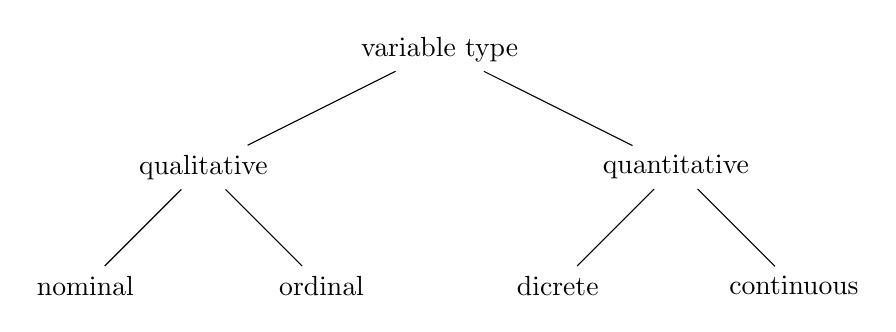
\begin{tikzpicture}[
    %sibling distance=10em,
    level 1/.style={sibling distance=60mm},
    level 2/.style={sibling distance=30mm}
    %   level 2/.style={shape=rectangle, rounded corners,
    %    draw, align=center,
    %    top color=white, bottom color=blue!20}
   ]
   \node {variable type}
   child { node {qualitative}
     child { node {nominal}}
     child { node {ordinal}}
    }
   child { node {quantitative}
     child { node {dicrete}}
     child { node {continuous}}
    };
   %        child { node {relation sign} }
   %        child { node {several places} }
  \end{tikzpicture}
 \end{center}

\end{document}
